% Notas de la comparación con otros criterios de selección (14 de octubre de 2026).
% Tablas: tables/tableS_*.tex (certificados/tablas_suplemento.py);
% figuras: figures/figS_*.pdf (certificados/figuras_suplemento.py).

\snote{profile}

\subsection*{Purpose}
Profile likelihood (Raue et al., 2009) is the standard method to assess which parameters the data determine, and profile-likelihood-based reduction (Maiwald et al., 2016) uses it to decide which parameters to fix. We computed the profile of every biological parameter of every problem in which it was feasible, for two purposes: as an independent estimate of how many parameters the data determine, and as one of the four criteria with which our selection is compared (main text, \emph{Comparison with existing selection criteria}).

\subsection*{Design}
\begin{enumerate}\itemsep0pt
\item The full model (all free parameters) was re-estimated on the training data of the external validation, from $\theta_0$, giving $\hat\theta_{\mathrm{train}}$ and the minimum $\chi^2_{\min}$. The finite-difference Jacobian of this fit was evaluated in parallel.
\item For each biological parameter $j$, $\log|\theta_j|$ was fixed at $\log|\hat\theta_{\mathrm{train},j}|\pm\{0.1,0.3,0.6,1.2,2.3\}$ (up to a factor of 10), within the same bounds $[|\theta_0|/10,10|\theta_0|]$ as all other fits, and all other free parameters were re-estimated from $\hat\theta_{\mathrm{train}}$; $\Delta\chi^2=\chi^2-\chi^2_{\min}$. All points of a problem were computed in parallel. Points whose fit failed (simulation failure, $\Delta\chi^2>10^4$) were excluded.
\item If a profile point improved the minimum by more than one unit of $\chi^2$, the full model had not converged: it was re-estimated from that point and all profiles were recomputed (at most three times; ten for Raia, which converged after four).
\item A parameter is \emph{identifiable} if its profile exceeds $\Delta\chi^2=3.84$ (95\%, one degree of freedom) on both sides, \emph{bounded on one side} if only on one side, and \emph{flat} otherwise. For the comparison, the $k=|S|$ parameters with the narrowest profile confidence interval were selected.
\end{enumerate}
The computation requires repeated re-estimation of the full model and was feasible for the 26 problems with at most 60 free parameters; Bachmann (90), Lucarelli (72), Raimundez (126), Chen (155) and Lang (277) were not evaluated, nor Blasi, which has no training/test split.

\subsection*{Results}
Supplementary Table~\ref{tab:perfil} gives the classification of every problem. The median number of identifiable biological parameters was 2 (17\% of the biological parameters); six problems had none and 14 of the 26 had two or fewer. This agrees with the size of the subsets selected by our method, obtained by a different principle. The selected parameters, however, rarely coincide (Supplementary Table~\ref{tab:selecciones}): a flat profile means that other free parameters can compensate for changes in the profiled parameter, whereas our method asks which parameters suffice when all others are fixed at $\theta_0$. Supplementary Figure~\ref{fig:perfiles} shows the profiles of three problems. Three problems needed re-estimations of the optimum (Borghans, Okuonghae, Raia), which shows that the full-model fit from $\theta_0$ on the training data had not converged; Isensee kept a residual improvement of 1.16 after its three re-estimations, slightly above the criterion of one unit.

{\footnotesize\setlength{\tabcolsep}{4pt}
\begin{longtable}{@{}lrrrrrp{5.2cm}rl@{}}
\caption{Profile likelihood of the biological parameters (training data). Ident.: profile above $\Delta\chi^2=3.84$ on both sides; one side: only on one side; flat: on neither side. Selected: the $k$ parameters with the narrowest profile confidence interval. Common: parameters shared with the subset of our method. Re-fits: times the full model was re-estimated because a profile point improved the optimum; residual: remaining improvement (in units of $\chi^2$) after the last re-fit.}\label{tab:perfil}\\
\toprule
Problem & $k$ & Bio & Ident. & One side & Flat & Selected by profile likelihood & Common & Note \\
\midrule
\endfirsthead
\multicolumn{9}{@{}l}{\emph{(continued)}}\\
\toprule
Problem & $k$ & Bio & Ident. & One side & Flat & Selected by profile likelihood & Common & Note \\
\midrule
\endhead
Alkan & 2 & 34 & 14 & 9 & 11 & kt, k\_death\_reox & 1 & -- \\
Armistead & 2 & 10 & 1 & 0 & 9 & k\_d, k2 & 1 & -- \\
Bachmann & \multicolumn{8}{l}{\emph{not evaluated: 90 free parameters > PL\_PMAX=60}} \\
Bertozzi & 2 & 3 & 1 & 1 & 1 & I0\_CA, R0\_CA & 0 & -- \\
Blasi & \multicolumn{8}{l}{\emph{not evaluated: no training/test split}} \\
Boehm & 2 & 6 & 1 & 3 & 2 & k\_phos, k\_exp\_homo & 1 & -- \\
Borghans & 2 & 20 & 17 & 2 & 1 & Kz, v0 & 1 & 3 re-fits; residual 1.56 \\
Brannmark & 2 & 15 & 0 & 2 & 13 & k\_IRSiP\_DosR, km2 & 1 & -- \\
Bruno & 5 & 10 & 9 & 0 & 1 & init\_bcar1, kb1, init\_bcry\_1, init\_b10\_1, kc2 & 3 & -- \\
Chen & \multicolumn{8}{l}{\emph{not evaluated: 155 free parameters > PL\_PMAX=60}} \\
Elowitz & 2 & 18 & 3 & 1 & 14 & n\_Hill, tau\_prot\_GFP & 1 & -- \\
Fiedler & 2 & 12 & 0 & 3 & 9 & K\_2, k6 & 1 & -- \\
Fujita & 2 & 16 & 7 & 2 & 7 & reaction\_8\_k1, EGFR\_turnover & 0 & -- \\
Giordano & 2 & 43 & 0 & 0 & 43 & nu\_0, rho\_22 & 0 & -- \\
Isensee & 2 & 32 & 23 & 3 & 6 & kf\_RIIp\_2\_\_RII\_2, kf\_RII\_C\_2\_\_RIIp\_C\_2 & 0 & 3 re-fits; residual 1.16 \\
Lang & \multicolumn{8}{l}{\emph{not evaluated: 277 free parameters > PL\_PMAX=60}} \\
Laske & 2 & 6 & 0 & 2 & 4 & k\_bind\_M1, k\_syn\_R\_M & 1 & -- \\
Liu & 2 & 7 & 2 & 0 & 5 & kappa, rho & 1 & -- \\
Lucarelli & \multicolumn{8}{l}{\emph{not evaluated: 72 free parameters > PL\_PMAX=60}} \\
Okuonghae & 2 & 14 & 3 & 9 & 2 & sigma, nu & 0 & 2 re-fits \\
Oliveira & 2 & 12 & 2 & 6 & 4 & t\_1, beta\_1 & 0 & -- \\
Perelson & 2 & 2 & 0 & 0 & 2 & c, delta & 2 & -- \\
Rahman & 2 & 9 & 0 & 1 & 8 & behavioural\_change\_rate, infected\_normal\_worsen\_rate & 1 & -- \\
Raia & 2 & 18 & 5 & 13 & 0 & pSTAT5\_dephosphorylation, pJAK2\_dephosphorylation & 0 & 4 re-fits \\
Raimundez & \multicolumn{8}{l}{\emph{not evaluated: 126 free parameters > PL\_PMAX=60}} \\
Salazar-Cavazos & 2 & 6 & 4 & 0 & 2 & ratio\_kpkd\_YN\_\_FREE, kdephosYN\_\_FREE & 1 & -- \\
Schwen & 2 & 13 & 1 & 4 & 8 & ini\_R2fold, ini\_R1 & 2 & -- \\
Smith & 2 & 16 & 6 & 9 & 1 & kminus7b, k30r & 1 & -- \\
Sneyd & 2 & 14 & 2 & 3 & 9 & l4, k\_3 & 1 & -- \\
Weber & 2 & 26 & 1 & 11 & 14 & pu5, m22 & 0 & -- \\
Zhao & 3 & 21 & 3 & 5 & 13 & R\_Stage\_II\_Hubei, R\_Stage\_II\_China, gamma\_2\_Stage\_III\_Wuhan & 0 & -- \\
Zheng & 2 & 45 & 4 & 0 & 41 & k02\_01, k01\_02 & 1 & -- \\
\bottomrule
\end{longtable}

}

\begin{figure}[H]
\centering
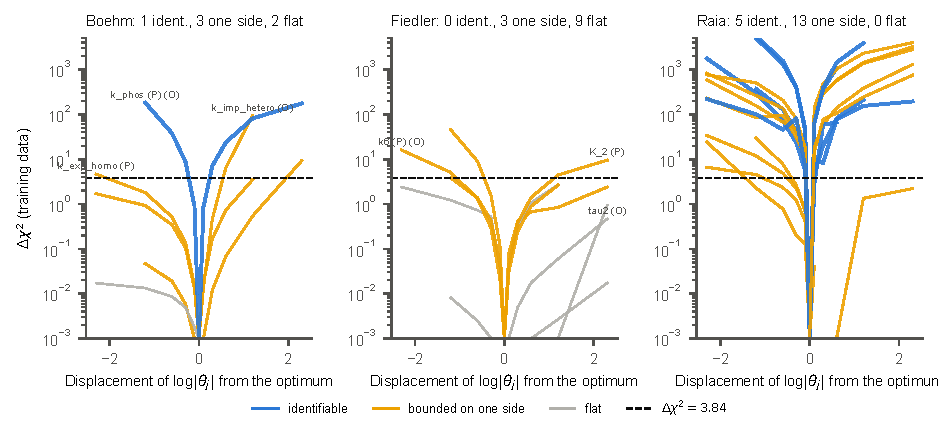
\includegraphics[width=\textwidth]{figures/figS_perfiles.pdf}
\caption{\textbf{Profile likelihoods of three problems.} $\Delta\chi^2$ on the training data as a function of the displacement of $\log|\theta_j|$ from the optimum, for every biological parameter, coloured by class. Dashed line, 95\% threshold. Labels mark the parameters selected by profile likelihood (P) and by our method (O); in Raia they are omitted for legibility.}
\label{fig:perfiles}
\end{figure}

\snote{morrisbrun}

\subsection*{Purpose}
The main text cites two further families of selection criteria: indices based on the collinearity of the sensitivity matrix, whose reference method is that of Brun \emph{et al.} (Brun et al., 2001), and global sensitivity screening, of which Morris's method (Morris, 1991) is the most widely used. We implemented both with the same protocol as the other criteria.

\subsection*{Design}
\emph{Brun.} Dimensionless sensitivities $s_{ij}=\theta_j\,\partial y_i/\partial\theta_j$ on the training outputs (forward differences with relative step $10^{-4}$), importance $\delta^{\mathrm{msqr}}_j=\|s_{:,j}\|/\sqrt n$, collinearity index $\gamma_K=1/\sqrt{\lambda_{\min}(\tilde S_K^\top\tilde S_K)}$ of the column-normalised subset and determinant measure $\rho_K=\det(S_K^\top S_K)^{1/(2k)}$. Among the 15 most important parameters, every $k$-subset was evaluated and the one with $\gamma_K\le10$ and the largest $\rho_K$ was selected (the one with the smallest $\gamma_K$ if none satisfies the bound). The importance $\delta^{\mathrm{msqr}}_j$ orders the parameters as the energy $E_j$ of our method; the difference lies in the selection rule and in the absence of a re-estimation test.

\emph{Morris.} Ten trajectories (seed 42) on a four-level grid of $\log|\theta_j|$ within $[\theta_0/10,10\theta_0]$ for the biological parameters (calibration parameters at $\theta_0$), step $\Delta=2/3$ of the range; elementary effect $\mathrm{EE}_j=\|y(x+\Delta e_j)-y(x)\|/\Delta$ on the training outputs; the $k$ parameters with the largest $\mu^\ast_j=\mathrm{mean}|\mathrm{EE}_j|$ were selected.

Chen and Lang were not included, because the sensitivity computations alone would take hours, as in the pivoted-QR comparison. Supplementary Table~\ref{tab:selecciones} lists the parameters selected by all five criteria.

{\scriptsize\setlength{\tabcolsep}{3pt}
\begin{longtable}{@{}l>{\raggedright}p{2.6cm}>{\raggedright}p{2.6cm}>{\raggedright}p{2.6cm}>{\raggedright}p{2.6cm}>{\raggedright\arraybackslash}p{2.6cm}@{}}
\caption{Biological parameters selected by each criterion (same number $k$ for all). --, criterion not computed for the problem.}\label{tab:selecciones}\\
\toprule
Problem & Ours & Pivoted QR & Brun & Morris & Profile likelihood \\
\midrule
\endfirsthead
\multicolumn{6}{@{}l}{\emph{(continued)}}\\
\toprule
Problem & Ours & Pivoted QR & Brun & Morris & Profile likelihood \\
\midrule
\endhead
Alkan & kt, k\_rep\_nhej & p\_chk1\_dea\_wip1, k\_death\_reox & kt, p\_atm\_act\_dsb & kt, k\_damage\_sn38\_ssb & kt, k\_death\_reox \\
Armistead & k\_d, alpha\_cer & k00, k2 & k\_d, k00 & k00, k\_d & k\_d, k2 \\
Bachmann & CISRNADelay, JAK2ActEpo & SOCS3Inh, CISEqcOE & STAT5Imp, JAK2ActEpo & CISRNADelay, JAK2ActEpo & -- \\
Bertozzi & R0\_NY, I0\_NY & R0\_CA, I0\_CA & R0\_CA, I0\_CA & gamma\_CA, R0\_CA & I0\_CA, R0\_CA \\
Blasi & a\_basal, a\_k16\_k12k16 & -- & -- & -- & -- \\
Boehm & k\_imp\_hetero, k\_phos & k\_phos, k\_imp\_homo & k\_phos, k\_imp\_hetero & k\_phos, k\_imp\_hetero & k\_phos, k\_exp\_homo \\
Borghans & Kz, K\_par & Kd, init\_A\_state & K\_par, Vm2 & K\_par, beta\_par & Kz, v0 \\
Brannmark & k1f, km2 & k1a, k\_IRSiP\_DosR & k1f, k1a & k22, k3 & k\_IRSiP\_DosR, km2 \\
Bruno & kb1, init\_bcar2, init\_zea\_1, init\_bcar1, init\_bcry\_1 & init\_b10\_1, init\_bcar1, kc4, kc1, kc2 & init\_bcar1, kb1, init\_bcry\_1, init\_b10\_1, kc2 & init\_bcry\_1, init\_b10\_1, init\_bcar1, kb2, kc2 & init\_bcar1, kb1, init\_bcry\_1, init\_b10\_1, kc2 \\
Chen & k106, k44 & -- & -- & -- & -- \\
Elowitz & n\_Hill, tau\_mRNA & eff\_GFP, tau\_prot\_GFP & n\_Hill, tau\_mRNA & n\_Hill, tau\_prot\_GFP & n\_Hill, tau\_prot\_GFP \\
Fiedler & tau2, k6 & k11, k5 & tau2, k5 & K\_1, tau2 & K\_2, k6 \\
Fujita & init\_AKT, reaction\_6\_k1 & reaction\_1\_k1, reaction\_6\_k1 & init\_AKT, reaction\_6\_k1 & reaction\_6\_k1, reaction\_8\_k1 & reaction\_8\_k1, EGFR\_turnover \\
Giordano & alpha\_4, alpha\_28 & delta\_0, eta\_0 & alpha\_4, alpha\_22 & alpha\_4, alpha\_0 & nu\_0, rho\_22 \\
Isensee & kf\_RIIp\_C\_2\_\_RII\_C\_2, xi\_kf\_RII\_C\_2\_\_RII\_2 & kf\_Fsk, KD\_H89 & kf\_RII\_C\_2\_\_RIIp\_C\_2, xi\_kf\_RII\_C\_2\_\_RII\_2 & kf\_RII\_C\_2\_\_RIIp\_C\_2, kf\_RIIp\_2\_\_RII\_2 & kf\_RIIp\_2\_\_RII\_2, kf\_RII\_C\_2\_\_RIIp\_C\_2 \\
Lang & kDeE2f1, kDeCe & -- & -- & -- & -- \\
Laske & k\_imp, k\_syn\_R\_M & k\_imp, k\_rel & k\_syn\_R\_M, k\_bind\_M1 & k\_syn\_R\_M, k\_bind\_M1 & k\_bind\_M1, k\_syn\_R\_M \\
Liu & kappa, phi & kappa, rho & kappa, rho & kappa, rho & kappa, rho \\
Lucarelli & init\_Rec, S2tot, S3tot, S\_dephosphos, S\_phos, geneF\_turn, k\_234, geneK\_turn, S4tot, geneH\_turn & S4tot, geneK\_turn, geneJ\_turn, geneB\_act2, geneG\_act1, geneH\_turn, geneL\_turn, geneE\_act2, geneI\_act1, geneC\_act1 & init\_Rec, S2tot, S\_dephosphos, S\_phos, Rec\_act, geneF\_turn, k\_234, geneK\_turn, geneH\_turn, geneG\_turn & init\_Rec, S3tot, S2tot, pRec\_degind, S\_dephosphos, S\_phos, geneF\_turn, geneF\_act1, Rec\_act, geneF\_inh1 & -- \\
Okuonghae & transmission\_rate\_effective, gamma\_i & asymptomatic\_start, d\_D & transmission\_rate\_effective, psi & sigma, nu & sigma, nu \\
Oliveira & beta\_0, h\_hosp\_rate & beta\_1, symptomatic\_init\_concentration & beta\_0, t\_1 & beta\_0, t\_1 & t\_1, beta\_1 \\
Perelson & c, delta & c, delta & c, delta & c, delta & c, delta \\
Rahman & infected\_moderate\_transmission\_rate, infected\_normal\_worsen\_rate & infected\_moderate\_transmission\_rate, treated\_moderate\_improve\_rate & infected\_moderate\_transmission\_rate, behavioural\_change\_rate & infected\_normal\_transmission\_rate\_relative, infected\_moderate\_transmission\_rate & behavioural\_change\_rate, infected\_normal\_worsen\_rate \\
Raia & SOCS3mRNA\_production, init\_Rec\_i & Rec\_recycle, DecoyR\_binding & SOCS3mRNA\_production, init\_Rec\_i & SOCS3mRNA\_production, Rec\_recycle & pSTAT5\_dephosphorylation, pJAK2\_dephosphorylation \\
Raimundez & kdeg\_membran\_\_MKN1, d\_kimp\_pEGFR\_EGF\_2\_\_MKN1\_2\_HS746T & d\_MAPKtotal\_\_MKN1\_2\_HS746T, d\_MPI3Ktotal\_\_fm\_2\_hm & kdeg\_membran\_\_MKN1, ka\_MAPK\_\_MKN1 & d\_AKTtotal\_\_fm\_2\_hm, ki\_AKT\_\_MKN1 & -- \\
Salazar-Cavazos & ratio\_kpkd\_Y1068\_\_FREE, ratio\_kpkd\_YN\_\_FREE & GRB2\_total\_\_FREE, kdephosYN\_\_FREE & ratio\_kpkd\_Y1068\_\_FREE, ratio\_kpkd\_YN\_\_FREE & ratio\_kpkd\_Y1068\_\_FREE, ratio\_kpkd\_YN\_\_FREE & ratio\_kpkd\_YN\_\_FREE, kdephosYN\_\_FREE \\
Schwen & ini\_R1, ini\_R2fold & kd2fold, kout & ini\_R1, kon\_unspec & ini\_R2fold, ini\_R1 & ini\_R2fold, ini\_R1 \\
Smith & k8, kminus7b & kminus7a, k43r & k8, k30f & kminus8, kminus7b & kminus7b, k30r \\
Sneyd & l4, l2 & k\_2, k\_3 & l4, l2 & l2, k4 & l4, k\_3 \\
Weber & s12, a21 & a22, pu5 & a21, s12 & pu3, a21 & pu5, m22 \\
Zhao & R\_Stage\_I\_China, R\_Stage\_II\_Wuhan, gamma\_1\_Stage\_I\_Hubei & R\_Stage\_I\_Wuhan, R\_Stage\_III\_Wuhan, R\_Stage\_II\_Hubei & R\_Stage\_I\_China, gamma\_1\_Stage\_I\_Wuhan, R\_Stage\_II\_Hubei & R\_Stage\_I\_China, gamma\_2\_Stage\_I\_China, R\_Stage\_II\_China & R\_Stage\_II\_Hubei, R\_Stage\_II\_China, gamma\_2\_Stage\_III\_Wuhan \\
Zheng & k01\_02, k13\_12 & k01\_11, k10\_00 & k01\_11, k12\_13 & k01\_02, k12\_13 & k02\_01, k01\_02 \\
\bottomrule
\end{longtable}

}

\snote{compreal}

Supplementary Table~\ref{tab:realdata} gives the test $\chi^2/n$ on the held-out experiments of every criterion and baseline, together with the full model and the published estimate, and Supplementary Table~\ref{tab:wilcoxonreal} the paired comparison with our method over problems. When the non-selected parameters are kept at $\theta_0$, all selection criteria and the random and calibration-only baselines predict similarly: the median ratios to our method are between 0.98 and 1.00, and only pivoted QR (1\% lower $\chi^2$) and calibration-only re-estimation (2\% lower) differ significantly, in favour of the alternative. Oliveira is the only problem in which the specific selection matters strongly. As discussed in the main text, this test does not discriminate between criteria because the fixed parameters carry the information of $\theta_0$, which was estimated with all data.

{\scriptsize\setlength{\tabcolsep}{3pt}
\begin{longtable}{@{}lrrrrrrrrr@{}}
\caption{Test $\chi^2/n$ on the held-out experiments (real data) of every selection criterion and baseline. All variants keep the non-selected parameters at $\theta_0$ except the full model, which re-estimates all parameters on the training data. Bold: lowest value among the seven selection variants. $\theta_0$, published estimate, obtained using all data including the test experiments.}\label{tab:realdata}\\
\toprule
Problem & Ours & Calib. only & Random & QR (earlier) & Brun & Morris & Profile & Full & $\theta_0$ \\
\midrule
\endfirsthead
\multicolumn{10}{@{}l}{\emph{(continued)}}\\
\toprule
Problem & Ours & Calib. only & Random & QR (earlier) & Brun & Morris & Profile & Full & $\theta_0$ \\
\midrule
\endhead
Alkan & 2.75 & \textbf{2.72} & 2.72 & 2.73 & 2.74 & 2.86 & 2.74 & 3.37 & 2.47 \\
Armistead & 1.22 & \textbf{1.16} & 1.16 & 1.21 & 1.22 & 1.22 & 1.37 & 1.37 & 1.16 \\
Bachmann & 4.77 & 4.76 & 4.84 & \textbf{4.75} & 4.75 & 4.77 & 4.77 & 7.35 & 1.05 \\
Boehm & 2.57 & \textbf{0.341} & 1.09 & 0.349 & 2.57 & 2.57 & 0.425 & 11.2 & 0.341 \\
Borghans & 0.743 & 0.778 & 0.768 & 0.776 & \textbf{0.742} & 0.743 & 0.744 & 0.744 & 0.74 \\
Brannmark & 5.96 & \textbf{0.938} & 2.95 & 0.951 & 1.17 & 147 & 1.82 & 6,277 & 0.938 \\
Bruno & 0.909 & \textbf{0.909} & 0.911 & 0.911 & 0.909 & 0.911 & 0.909 & 208 & 0.909 \\
Chen & \textbf{20.9} & -- & -- & -- & -- & -- & -- & 17.7 & 15.2 \\
Elowitz & 1.5 & \textbf{1.39} & 1.44 & 1.41 & 1.5 & 1.43 & 1.43 & 3.89 & 1.38 \\
Fiedler & 11.2 & 11.7 & 11.2 & 10.9 & 11 & 11.1 & \textbf{9.56} & 9.32 & 1.22 \\
Fujita & 5.94 & \textbf{5.94} & 6.02 & 5.94 & 5.94 & 5.94 & 5.98 & 8.03 & 5.63 \\
Giordano & $1.0\times10^{-7}$ & $7.4\times10^{-9}$ & $8.7\times10^{-9}$ & \textbf{$7.2\times10^{-9}$} & $2.7\times10^{-8}$ & $1.3\times10^{-8}$ & $1.4\times10^{-8}$ & 0.00773 & $7.4\times10^{-9}$ \\
Isensee & 1.08 & 1.08 & 1.08 & 1.08 & 1.08 & \textbf{1.08} & 1.08 & 1.08 & 1.04 \\
Laske & 0.758 & 0.445 & 0.445 & 0.445 & \textbf{0.445} & \textbf{0.445} & \textbf{0.445} & 1.87 & 0.445 \\
Liu & 0.954 & \textbf{0.942} & 0.942 & 1.03 & 1.03 & 1.03 & 1.03 & 1.02 & 0.942 \\
Lucarelli & 1.66 & \textbf{1.02} & 1.06 & 1.07 & 1.02 & 1.03 & 1.08 & 3.34 & 1.02 \\
Okuonghae & $4.7\times10^{4}$ & \textbf{$2.9\times10^{4}$} & $5.6\times10^{4}$ & $3.2\times10^{4}$ & $8.0\times10^{4}$ & $5.1\times10^{4}$ & $5.1\times10^{4}$ & $1.2\times10^{5}$ & $2.9\times10^{4}$ \\
Oliveira & 912 & $4.6\times10^{5}$ & $2.0\times10^{4}$ & $7.3\times10^{4}$ & \textbf{553} & \textbf{553} & $3.0\times10^{5}$ & $8.1\times10^{4}$ & $4.6\times10^{5}$ \\
Perelson & \textbf{$4.0\times10^{-13}$} & \textbf{$4.0\times10^{-13}$} & \textbf{$4.0\times10^{-13}$} & \textbf{$4.0\times10^{-13}$} & \textbf{$4.0\times10^{-13}$} & \textbf{$4.0\times10^{-13}$} & \textbf{$4.0\times10^{-13}$} & $4.0\times10^{-13}$ & $4.0\times10^{-13}$ \\
Rahman & 0.00199 & \textbf{0.00148} & 0.00171 & 0.00154 & 0.00247 & 0.00163 & 0.00272 & 0.0257 & 0.00148 \\
Raia & 8.22 & \textbf{0.439} & 2.21 & 7.24 & 8.23 & 8.15 & 0.799 & 5.1 & 0.417 \\
Raimundez & 1.17 & \textbf{1.17} & 1.18 & 1.17 & 1.17 & 1.17 & -- & 1.43 & 0.98 \\
Salazar-Cavazos & 102 & \textbf{96.9} & 103 & 102 & 102 & 102 & 119 & 124 & 96.9 \\
Schwen & 8.2 & \textbf{8.06} & 8.35 & 8.43 & 8.3 & 8.2 & 8.2 & 8.4 & 0.768 \\
Smith & $1.5\times10^{4}$ & $1.6\times10^{4}$ & $1.6\times10^{4}$ & $1.5\times10^{4}$ & \textbf{$1.4\times10^{4}$} & $1.5\times10^{4}$ & $1.5\times10^{4}$ & $1.5\times10^{4}$ & $8.3\times10^{4}$ \\
Sneyd & 2.22 & \textbf{1.37} & 1.89 & 1.48 & 2.22 & 2.18 & 1.52 & 2.56 & 1.37 \\
Weber & 1 & 0.997 & 1.01 & \textbf{0.997} & 1 & 45.6 & 0.997 & 16 & 0.993 \\
Zhao & \textbf{0.345} & 0.345 & 0.345 & 0.345 & 0.345 & 0.345 & 0.345 & 0.345 & 0.345 \\
Zheng & 1.58 & \textbf{1.51} & 1.52 & 1.55 & 1.59 & 1.58 & 3.16 & 20.8 & 1.51 \\
\bottomrule
\end{longtable}

}

{\small
\begin{longtable}{@{}lrrrrrr@{}}
\caption{Real data: paired comparison of the test $\chi^2/n$ of our method with each alternative over problems. Better/worse: our method lower/higher by more than 5\%; equal: within 5\%. Median ratio: alternative over ours (below 1, the alternative predicts better). $p$: two-sided Wilcoxon signed-rank test on the log ratios.}\label{tab:wilcoxonreal}\\
\toprule
Our method compared with & Problems & Ours better & Ours worse & Equal & Median ratio & $p$ \\
\midrule
\endfirsthead
\multicolumn{7}{@{}l}{\emph{(continued)}}\\
\toprule
Our method compared with & Problems & Ours better & Ours worse & Equal & Median ratio & $p$ \\
\midrule
\endhead
Pivoted QR & 28 & 2 & 10 & 16 & 0.99 & 0.026 \\
Brun & 28 & 3 & 5 & 20 & 1.00 & 0.27 \\
Morris & 28 & 4 & 6 & 18 & 1.00 & 0.46 \\
Profile likelihood & 27 & 7 & 9 & 11 & 1.00 & 0.44 \\
Random subsets (median of 20) & 28 & 3 & 9 & 16 & 1.00 & 0.27 \\
Calibration only ($k=0$) & 28 & 2 & 13 & 13 & 0.99 & 0.0027 \\
Full model re-estimated on training data & 29 & 20 & 3 & 6 & 1.23 & 8.2e-05 \\
Reduced model, nested without $\theta_0$ anchor & 29 & 21 & 3 & 5 & 1.35 & 7.2e-05 \\
Published estimate $\theta_0$ & 29 & 2 & 20 & 7 & 0.90 & 0.00022 \\
\bottomrule
\end{longtable}

}

Supplementary Table~\ref{tab:controls} classifies every problem according to how our method, pivoted QR and the two baselines compare.

\begin{table}[H]
\caption{External validation against three baseline selectors, with a classification of each problem. Test $\chi^2/n$ of our method, of calibration-only re-estimation ($|S|=0$), of pivoted QR and of random biological subsets of the same size $k$ (median over 20 draws). Category: \textbf{S}, sloppy---all four values within 10\% of each other; \textbf{C}, calibration dominates (bold, lowest value); \textbf{O}, our method clearly best; \textbf{P}, all methods near zero ($<$0.01); \textbf{F}, all methods fail ($\chi^2/n\gg1$).}
\label{tab:controls}
\centering
\small
\begin{tabular}{@{}lrccccc@{}}
\toprule
Problem & $k$ & $\chi^2_{\mathrm{ours}}$ & $\chi^2_{\mathrm{vac}}$ & $\chi^2_{\mathrm{QR}}$ & $\chi^2_{\mathrm{rand}}$ & Cat. \\
\midrule
Alkan        & 2  & 2.748 & 2.720 & 2.727 & 2.722 & S \\
Armistead    & 2  & 1.218 & 1.157 & 1.207 & 1.159 & S \\
Bachmann     & 2  & 4.768 & 4.759 & 4.746 & 4.845 & S \\
Boehm        & 2  & 2.567 & \textbf{0.341} & \textbf{0.349} & 1.095 & C \\
Borghans     & 2  & 0.743 & 0.778 & 0.776 & 0.768 & S \\
Brannmark    & 2  & 5.956 & \textbf{0.938} & \textbf{0.951} & 2.952 & C \\
Bruno        & 5  & 0.909 & 0.909 & 0.911 & 0.911 & S \\
Elowitz      & 2  & 1.498 & 1.391 & 1.407 & 1.439 & S \\
Fiedler      & 2  & 11.21 & 11.73 & 10.95 & 11.22 & S \\
Fujita       & 2  & 5.939 & 5.937 & 5.941 & 6.022 & S \\
Giordano     & 2  & $<$0.01 & $<$0.01 & $<$0.01 & $<$0.01 & P \\
Isensee      & 2  & 1.082 & 1.081 & 1.081 & 1.081 & S \\
Laske        & 2  & 0.758 & \textbf{0.445} & \textbf{0.445} & \textbf{0.445} & C \\
Liu          & 2  & 0.954 & 0.942 & 1.026 & 0.942 & S \\
Lucarelli    & 10 & 1.659 & \textbf{1.015} & 1.073 & 1.059 & C \\
Okuonghae    & 2  & $4.7\times10^4$ & $2.9\times10^4$ & $3.2\times10^4$ & $5.6\times10^4$ & F \\
Oliveira     & 2  & \textbf{912} & $4.6\times10^5$ & $7.3\times10^4$ & $2.0\times10^4$ & O \\
Perelson     & 2  & $<$0.01 & $<$0.01 & $<$0.01 & $<$0.01 & P \\
Rahman       & 2  & $<$0.01 & $<$0.01 & $<$0.01 & $<$0.01 & P \\
Raia         & 2  & 8.224 & \textbf{0.439} & 7.236 & 2.213 & C \\
Raimundez    & 2  & 1.188 & 1.167 & 1.168 & 1.181 & S \\
Salazar-C.   & 2  & 101.8 & 96.93 & 101.7 & 103.2 & F \\
Schwen       & 2  & 8.196 & 8.063 & 8.432 & 8.353 & S \\
Smith        & 2  & $1.5\times10^4$ & $1.6\times10^4$ & $1.5\times10^4$ & $1.6\times10^4$ & F \\
Sneyd        & 2  & 2.222 & \textbf{1.373} & 1.480 & 1.890 & C \\
Weber        & 2  & 1.001 & 0.997 & 0.997 & 1.014 & S \\
Zhao         & 3  & 0.345 & 0.345 & 0.345 & 0.345 & P \\
Zheng        & 2  & 1.582 & 1.505 & 1.553 & 1.521 & S \\
\bottomrule
\end{tabular}
\end{table}

\snote{admisother}

\subsection*{Purpose}
Our method returns a subset only if re-estimating it reproduces the full model under random parameter changes (admissibility). This note applies exactly the same test to the subsets of the other criteria, to determine whether they have this property without being selected for it.

\subsection*{Design}
The test replicates the code of the method: 15 scenarios $\theta^{(k)}=\theta_0\odot(1+\varepsilon u^{(k)})$ with the same seed (42), re-estimation of the subset together with the calibration parameters from two starting points, scenarios with non-finite outputs discarded, and the subset is admissible if the smaller of the median $e_{\mathrm{fit}}$ and the median $e_{\mathrm{rel}}$ is at most $\tau_e=0.436$ (with $|S|\ge2$). The eight problems that the method treats to first order were treated in the same way for every criterion. As a check, the test reproduces the published $e_{\mathrm{fit}}$ of our subsets (for example Armistead 0.117, Boehm 0.094, Fiedler 0.147). Because our subsets are selected by this test at $\varepsilon=0.05$, it was repeated at $\varepsilon=0.20$, a level used by none of the criteria.

\subsection*{Results}
Supplementary Table~\ref{tab:admis} and Supplementary Figure~\ref{fig:admismapa} give the result of every criterion in every problem, and Supplementary Table~\ref{tab:mcnemar} the paired comparison. At $\pm$5\% our subsets were admissible in all 29 problems, against 24 (Brun), 21 (Morris), 17 of 26 (profile likelihood) and 13 (pivoted QR); at $\pm$20\%, 28 of 29 against 23, 21, 17 of 26 and 14. There is no problem in which the subset of another criterion is admissible and ours is not. The only problem in which our subset loses admissibility at $\pm$20\% is Elowitz, one of the problems that are admissible with a small margin at $\pm$5\% (main text, \emph{Robustness}).

{\scriptsize
\begin{longtable}{@{}lrrrrr|rrrrr@{}}
\caption{Admissibility of the subsets of every criterion: smaller of the median $e_{\mathrm{fit}}$ and the median $e_{\mathrm{rel}}$ over 15 scenarios (the quantity compared with $\tau_e=0.436$ by the method), for parameter changes of $\pm$5\% (left) and $\pm$20\% (right). $\checkmark$, admissible. The eight problems that the method treats to first order are treated in the same way for every criterion.}\label{tab:admis}\\
\toprule
& \multicolumn{5}{c|}{$\pm$5\%} & \multicolumn{5}{c}{$\pm$20\%} \\
Problem & Ours & QR & Brun & Morris & Profile & Ours & QR & Brun & Morris & Profile \\
\midrule
\endfirsthead
\multicolumn{11}{@{}l}{\emph{(continued)}}\\
\toprule
& \multicolumn{5}{c|}{$\pm$5\%} & \multicolumn{5}{c}{$\pm$20\%} \\
Problem & Ours & QR & Brun & Morris & Profile & Ours & QR & Brun & Morris & Profile \\
\midrule
\endhead
Alkan & 0.12$^{\checkmark}$ & 0.95 & 0.13$^{\checkmark}$ & 0.12$^{\checkmark}$ & 0.13$^{\checkmark}$ & 0.13$^{\checkmark}$ & 0.94 & 0.13$^{\checkmark}$ & 0.12$^{\checkmark}$ & 0.14$^{\checkmark}$ \\
Armistead & 0.12$^{\checkmark}$ & 0.73 & 0.72 & 0.72 & 0.99 & 0.40$^{\checkmark}$ & 0.79 & 0.66 & 0.66 & 0.83 \\
Bachmann & 0.34$^{\checkmark}$ & 0.50 & 0.31$^{\checkmark}$ & 0.34$^{\checkmark}$ & -- & 0.32$^{\checkmark}$ & 0.50 & 0.31$^{\checkmark}$ & 0.32$^{\checkmark}$ & -- \\
Bertozzi & 0.33$^{\checkmark}$ & 0.94 & 0.94 & 0.94 & 0.94 & 0.43$^{\checkmark}$ & 0.91 & 0.91 & 0.91 & 0.91 \\
Boehm & 0.09$^{\checkmark}$ & 0.67 & 0.09$^{\checkmark}$ & 0.09$^{\checkmark}$ & 0.57 & 0.10$^{\checkmark}$ & 0.65 & 0.10$^{\checkmark}$ & 0.10$^{\checkmark}$ & 0.54 \\
Borghans & 0.04$^{\checkmark}$ & 0.53 & 0.17$^{\checkmark}$ & 0.36$^{\checkmark}$ & 0.10$^{\checkmark}$ & 0.17$^{\checkmark}$ & 0.34$^{\checkmark}$ & 0.20$^{\checkmark}$ & 0.31$^{\checkmark}$ & 0.19$^{\checkmark}$ \\
Brannmark & 0.08$^{\checkmark}$ & 0.12$^{\checkmark}$ & 0.10$^{\checkmark}$ & 0.11$^{\checkmark}$ & 0.09$^{\checkmark}$ & 0.08$^{\checkmark}$ & 0.11$^{\checkmark}$ & 0.10$^{\checkmark}$ & 0.11$^{\checkmark}$ & 0.08$^{\checkmark}$ \\
Bruno & 0.38$^{\checkmark}$ & 0.89 & 0.71 & 0.86 & 0.71 & 0.39$^{\checkmark}$ & 0.89 & 0.68 & 0.85 & 0.68 \\
Elowitz & 0.36$^{\checkmark}$ & 0.72 & 0.36$^{\checkmark}$ & 0.65 & 0.65 & 0.44 & 0.72 & 0.44 & 0.61 & 0.61 \\
Fiedler & 0.15$^{\checkmark}$ & 0.13$^{\checkmark}$ & 0.13$^{\checkmark}$ & 0.13$^{\checkmark}$ & 0.35$^{\checkmark}$ & 0.13$^{\checkmark}$ & 0.11$^{\checkmark}$ & 0.12$^{\checkmark}$ & 0.12$^{\checkmark}$ & 0.35$^{\checkmark}$ \\
Fujita & 0.29$^{\checkmark}$ & 0.18$^{\checkmark}$ & 0.29$^{\checkmark}$ & 0.27$^{\checkmark}$ & 0.22$^{\checkmark}$ & 0.25$^{\checkmark}$ & 0.15$^{\checkmark}$ & 0.25$^{\checkmark}$ & 0.25$^{\checkmark}$ & 0.21$^{\checkmark}$ \\
Giordano & 0.06$^{\checkmark}$ & 0.91 & 0.05$^{\checkmark}$ & 0.06$^{\checkmark}$ & 0.82 & 0.06$^{\checkmark}$ & 0.96 & 0.08$^{\checkmark}$ & 0.09$^{\checkmark}$ & 0.89 \\
Isensee & 0.08$^{\checkmark}$ & 0.10$^{\checkmark}$ & 0.10$^{\checkmark}$ & 0.10$^{\checkmark}$ & 0.10$^{\checkmark}$ & 0.06$^{\checkmark}$ & 0.10$^{\checkmark}$ & 0.10$^{\checkmark}$ & 0.10$^{\checkmark}$ & 0.10$^{\checkmark}$ \\
Laske & 0.10$^{\checkmark}$ & 0.12$^{\checkmark}$ & 0.15$^{\checkmark}$ & 0.15$^{\checkmark}$ & 0.15$^{\checkmark}$ & 0.11$^{\checkmark}$ & 0.13$^{\checkmark}$ & 0.15$^{\checkmark}$ & 0.15$^{\checkmark}$ & 0.15$^{\checkmark}$ \\
Liu & 0.26$^{\checkmark}$ & 0.27$^{\checkmark}$ & 0.27$^{\checkmark}$ & 0.27$^{\checkmark}$ & 0.27$^{\checkmark}$ & 0.25$^{\checkmark}$ & 0.15$^{\checkmark}$ & 0.15$^{\checkmark}$ & 0.15$^{\checkmark}$ & 0.15$^{\checkmark}$ \\
Lucarelli & 0.44$^{\checkmark}$ & 0.91 & 0.41$^{\checkmark}$ & 0.55 & -- & 0.43$^{\checkmark}$ & 0.91 & 0.42$^{\checkmark}$ & 0.55 & -- \\
Okuonghae & 0.04$^{\checkmark}$ & 0.11$^{\checkmark}$ & 0.04$^{\checkmark}$ & 0.04$^{\checkmark}$ & 0.04$^{\checkmark}$ & 0.05$^{\checkmark}$ & 0.17$^{\checkmark}$ & 0.03$^{\checkmark}$ & 0.03$^{\checkmark}$ & 0.03$^{\checkmark}$ \\
Oliveira & 0.13$^{\checkmark}$ & 0.04$^{\checkmark}$ & 0.08$^{\checkmark}$ & 0.08$^{\checkmark}$ & 0.05$^{\checkmark}$ & 0.14$^{\checkmark}$ & 0.04$^{\checkmark}$ & 0.06$^{\checkmark}$ & 0.06$^{\checkmark}$ & 0.06$^{\checkmark}$ \\
Perelson & 0.00$^{\checkmark}$ & 0.00$^{\checkmark}$ & 0.00$^{\checkmark}$ & 0.00$^{\checkmark}$ & 0.00$^{\checkmark}$ & 0.00$^{\checkmark}$ & 0.00$^{\checkmark}$ & 0.00$^{\checkmark}$ & 0.00$^{\checkmark}$ & 0.00$^{\checkmark}$ \\
Rahman & 0.04$^{\checkmark}$ & 0.11$^{\checkmark}$ & 0.04$^{\checkmark}$ & 0.08$^{\checkmark}$ & 0.04$^{\checkmark}$ & 0.04$^{\checkmark}$ & 0.12$^{\checkmark}$ & 0.05$^{\checkmark}$ & 0.07$^{\checkmark}$ & 0.04$^{\checkmark}$ \\
Raia & 0.03$^{\checkmark}$ & 0.04$^{\checkmark}$ & 0.03$^{\checkmark}$ & 0.03$^{\checkmark}$ & 0.05$^{\checkmark}$ & 0.03$^{\checkmark}$ & 0.04$^{\checkmark}$ & 0.03$^{\checkmark}$ & 0.03$^{\checkmark}$ & 0.06$^{\checkmark}$ \\
Raimundez & 0.37$^{\checkmark}$ & 0.53 & 0.52 & 0.53 & -- & 0.36$^{\checkmark}$ & 0.53 & 0.51 & 0.53 & -- \\
Salazar-Cavazos & 0.19$^{\checkmark}$ & 0.52 & 0.19$^{\checkmark}$ & 0.19$^{\checkmark}$ & 0.40$^{\checkmark}$ & 0.19$^{\checkmark}$ & 0.52 & 0.19$^{\checkmark}$ & 0.19$^{\checkmark}$ & 0.40$^{\checkmark}$ \\
Schwen & 0.17$^{\checkmark}$ & 0.19$^{\checkmark}$ & 0.19$^{\checkmark}$ & 0.17$^{\checkmark}$ & 0.17$^{\checkmark}$ & 0.18$^{\checkmark}$ & 0.17$^{\checkmark}$ & 0.18$^{\checkmark}$ & 0.18$^{\checkmark}$ & 0.18$^{\checkmark}$ \\
Smith & 0.08$^{\checkmark}$ & 0.09$^{\checkmark}$ & 0.08$^{\checkmark}$ & 0.08$^{\checkmark}$ & 0.06$^{\checkmark}$ & 0.07$^{\checkmark}$ & 0.09$^{\checkmark}$ & 0.08$^{\checkmark}$ & 0.07$^{\checkmark}$ & 0.06$^{\checkmark}$ \\
Sneyd & 0.38$^{\checkmark}$ & 0.74 & 0.38$^{\checkmark}$ & 0.50 & 0.68 & 0.35$^{\checkmark}$ & 0.73 & 0.35$^{\checkmark}$ & 0.51 & 0.68 \\
Weber & 0.04$^{\checkmark}$ & 0.48 & 0.04$^{\checkmark}$ & 0.04$^{\checkmark}$ & 0.07$^{\checkmark}$ & 0.04$^{\checkmark}$ & 0.54 & 0.04$^{\checkmark}$ & 0.04$^{\checkmark}$ & 0.08$^{\checkmark}$ \\
Zhao & 0.30$^{\checkmark}$ & 0.97 & 0.44 & 0.61 & 0.97 & 0.28$^{\checkmark}$ & 0.97 & 0.66 & 0.81 & 0.97 \\
Zheng & 0.30$^{\checkmark}$ & 0.70 & 0.29$^{\checkmark}$ & 0.29$^{\checkmark}$ & 0.67 & 0.30$^{\checkmark}$ & 0.58 & 0.30$^{\checkmark}$ & 0.28$^{\checkmark}$ & 0.57 \\
\midrule Admissible & 29/29 & 13/29 & 24/29 & 21/29 & 17/26 & 28/29 & 14/29 & 23/29 & 21/29 & 17/26 \\
\bottomrule
\end{longtable}

}

{\small
\begin{longtable}{@{}llrrrr@{}}
\caption{Admissibility of our subsets compared with those of each criterion: exact McNemar test over problems (problems in which only one of the two subsets is admissible).}\label{tab:mcnemar}\\
\toprule
Level & Criterion & Problems & Only ours admissible & Only the other & $p$ \\
\midrule
\endfirsthead
\multicolumn{6}{@{}l}{\emph{(continued)}}\\
\toprule
Level & Criterion & Problems & Only ours admissible & Only the other & $p$ \\
\midrule
\endhead
$\pm$5\% & Pivoted QR & 28 & 14 & 0 & 0.00012 \\
$\pm$5\% & Brun & 28 & 2 & 0 & 0.5 \\
$\pm$5\% & Morris & 28 & 5 & 0 & 0.062 \\
$\pm$5\% & Profile likelihood & 27 & 9 & 0 & 0.0039 \\
$\pm$20\% & Pivoted QR & 28 & 12 & 0 & 0.00049 \\
$\pm$20\% & Brun & 28 & 2 & 0 & 0.5 \\
$\pm$20\% & Morris & 28 & 4 & 0 & 0.12 \\
$\pm$20\% & Profile likelihood & 27 & 8 & 0 & 0.0078 \\
\bottomrule
\end{longtable}

}

\begin{figure}[H]
\centering
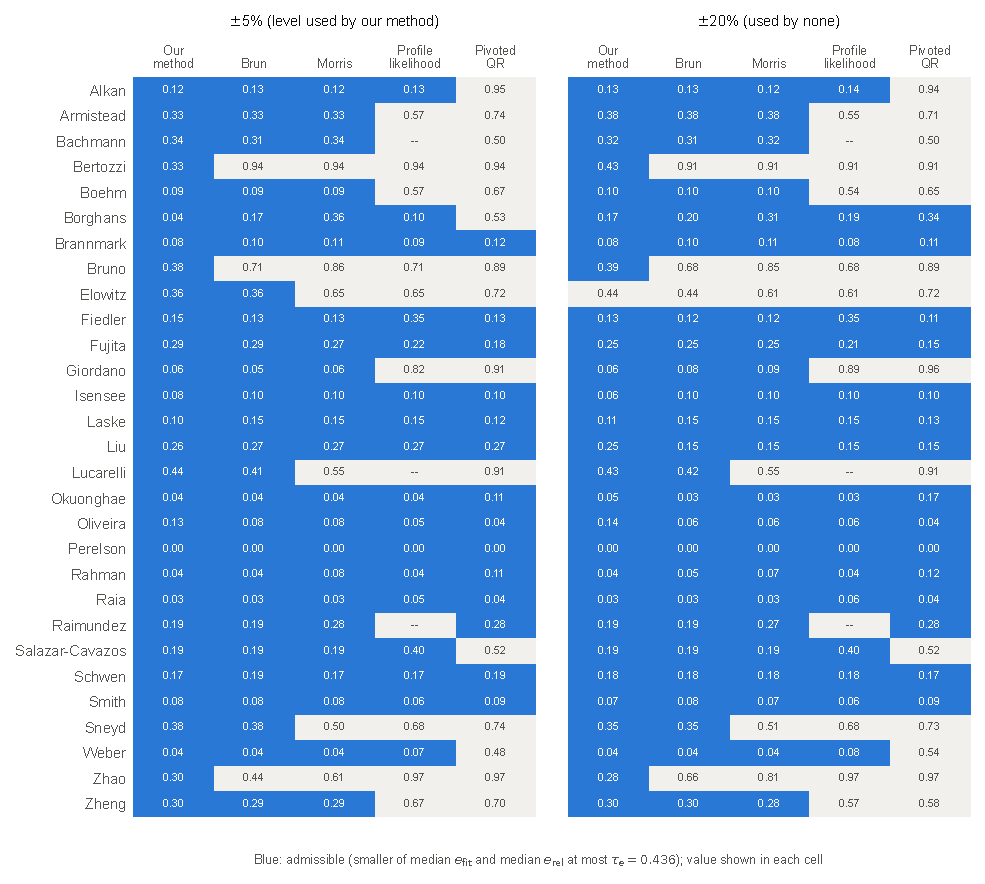
\includegraphics[width=0.92\textwidth]{figures/figS_admis_mapa.pdf}
\caption{\textbf{Admissibility of the subsets of every criterion in every problem.} Cell value: smaller of the median $e_{\mathrm{fit}}$ and the median $e_{\mathrm{rel}}$ over 15 scenarios; blue, admissible ($\le\tau_e=0.436$). Left, $\pm$5\%; right, $\pm$20\%. --, criterion not computed.}
\label{fig:admismapa}
\end{figure}

\snote{compsynth}

\subsection*{Design}
The synthetic prediction experiment (\sref{synth}) was repeated with the subsets of every criterion, with the same 20 seeds (42--61), so that the five criteria are evaluated on exactly the same truths and noise realisations. Each subset, with the calibration parameters, was re-estimated on the synthetic training data from $\theta_0$ and $e_{\mathrm{pred}}$ was computed on the test data. The comparison uses the cases common to the five criteria in which the parameter change exceeded the noise (280 cases in 23 problems). Because the 20 seeds of a problem are not independent, the main statistic resamples whole problems (Methods, \emph{Statistics}).

\subsection*{Results}
Supplementary Table~\ref{tab:synthmethods} gives the results per problem and Supplementary Table~\ref{tab:synthstats} the statistics. Our subsets reached $e_{\mathrm{pred}}\le\tau_e$ in 54\% of the cases, those of Brun in 55\%, Morris 48\%, profile likelihood 39\% and pivoted QR 34\%; the advantage of our method over pivoted QR (20 percentage points, 95\% confidence interval 7--33) and profile likelihood (15, 4--27) is significant, whereas the differences from Morris and Brun are not. The per-problem median prediction error did not differ significantly between criteria (Wilcoxon $p\ge0.08$). Supplementary Figure~\ref{fig:synthsemillas} shows that the ordering of the criteria is similar across seeds.

{\small
\begin{longtable}{@{}lrrrrrr@{}}
\caption{Synthetic prediction experiment for the five criteria (20 seeds, cases common to all criteria in which the parameter change exceeded the noise; the same cases as in Table~2 of the main text; pivoted QR in the standard Golub--Klema--Stewart form). Each entry: number of cases with $e_{\mathrm{pred}}\le\tau_e$ and, in parentheses, the median $e_{\mathrm{pred}}$.}\label{tab:synthmethods}\\
\toprule
Problem & Cases & Ours & Pivoted QR & Brun & Morris & Profile \\
\midrule
\endfirsthead
\multicolumn{7}{@{}l}{\emph{(continued)}}\\
\toprule
Problem & Cases & Ours & Pivoted QR & Brun & Morris & Profile \\
\midrule
\endhead
Alkan & 3 & 3 (0.21) & 0 (0.76) & 3 (0.28) & 3 (0.16) & 3 (0.28) \\
Armistead & 12 & 7 (0.42) & 6 (0.40) & 7 (0.42) & 7 (0.42) & 4 (0.65) \\
Bachmann & 2 & 0 (1.63) & 0 (1.42) & 0 (1.81) & 0 (1.36) & 0 (1.75) \\
Boehm & 4 & 1 (0.53) & 2 (0.43) & 1 (0.53) & 1 (0.53) & 0 (0.94) \\
Borghans & 11 & 2 (0.81) & 1 (0.91) & 1 (0.83) & 1 (0.83) & 1 (0.85) \\
Brannmark & 18 & 1 (1.84) & 1 (1.71) & 0 (1.23) & 0 (7.56) & 0 (0.99) \\
Bruno & 6 & 4 (0.34) & 0 (1.00) & 4 (0.34) & 0 (0.99) & 4 (0.34) \\
Elowitz & 17 & 11 (0.27) & 3 (0.63) & 11 (0.27) & 7 (0.54) & 7 (0.54) \\
Fiedler & 6 & 1 (1.00) & 1 (0.94) & 1 (1.00) & 1 (0.99) & 0 (1.68) \\
Fujita & 18 & 14 (0.31) & 17 (0.23) & 14 (0.31) & 14 (0.30) & 16 (0.24) \\
Isensee & 11 & 8 (0.15) & 11 (0.12) & 7 (0.15) & 6 (0.24) & 3 (0.94) \\
Liu & 1 & 0 (0.64) & 0 (0.50) & 0 (0.50) & 0 (0.50) & 0 (0.50) \\
Okuonghae & 20 & 17 (0.16) & 12 (0.41) & 18 (0.06) & 18 (0.09) & 18 (0.09) \\
Oliveira & 20 & 12 (0.39) & 6 (1.36) & 13 (0.35) & 13 (0.35) & 7 (0.63) \\
Perelson & 1 & 0 (20.95) & 0 (20.95) & 0 (20.95) & 0 (20.95) & 0 (20.95) \\
Rahman & 19 & 15 (0.12) & 16 (0.25) & 13 (0.13) & 13 (0.39) & 14 (0.23) \\
Raia & 8 & 7 (0.24) & 0 (1.01) & 7 (0.24) & 7 (0.23) & 0 (1.01) \\
Salazar-Cavazos & 18 & 12 (0.33) & 0 (0.92) & 12 (0.33) & 12 (0.33) & 2 (0.83) \\
Schwen & 9 & 0 (1.62) & 0 (1.62) & 0 (1.42) & 0 (1.62) & 0 (1.62) \\
Smith & 20 & 18 (0.10) & 8 (0.67) & 19 (0.11) & 18 (0.09) & 19 (0.11) \\
Sneyd & 1 & 1 (0.27) & 0 (0.98) & 1 (0.27) & 0 (0.88) & 1 (0.40) \\
Weber & 20 & 11 (0.36) & 0 (0.86) & 11 (0.36) & 2 (0.86) & 6 (0.59) \\
Zhao & 16 & 0 (1.00) & 0 (1.00) & 0 (1.00) & 0 (1.00) & 0 (1.00) \\
Zheng & 20 & 12 (0.41) & 0 (0.95) & 11 (0.42) & 11 (0.41) & 4 (0.72) \\
\midrule Total & 281 & 157 (56\%) & 84 (30\%) & 154 (55\%) & 134 (48\%) & 109 (39\%) \\
\bottomrule
\end{longtable}

}

{\small
\begin{longtable}{@{}lrrrrrr@{}}
\caption{Synthetic experiment, statistics over problems. Left: difference in the fraction of cases with $e_{\mathrm{pred}}\le\tau_e$ (ours minus criterion, percentage points) with a 95\% confidence interval and $p$-value from resampling whole problems with all their seeds (10,000 replicates). Right: per-problem median over seeds of the ratio $e_{\mathrm{pred}}$(criterion)/$e_{\mathrm{pred}}$(ours) (problems with at least 10 seeds), its median and the two-sided Wilcoxon $p$-value.}\label{tab:synthstats}\\
\toprule
Criterion & Difference & 95\% CI & $p$ & Problems & Median ratio & $p$ \\
\midrule
\endfirsthead
\multicolumn{7}{@{}l}{\emph{(continued)}}\\
\toprule
Criterion & Difference & 95\% CI & $p$ & Problems & Median ratio & $p$ \\
\midrule
\endhead
Pivoted QR & +19.6 & +6.5 to +32.5 & 0.003 & 28 & 1.01 & 0.24 \\
Brun & -1.1 & -7.6 to +3.5 & 0.82 & 28 & 1.00 & 0.14 \\
Morris & +6.1 & -3.2 to +15.4 & 0.21 & 28 & 1.00 & 0.54 \\
Profile likelihood & +15.0 & +4.3 to +26.5 & 0.0058 & 25 & 1.04 & 0.32 \\
\bottomrule
\end{longtable}

}

\begin{figure}[H]
\centering
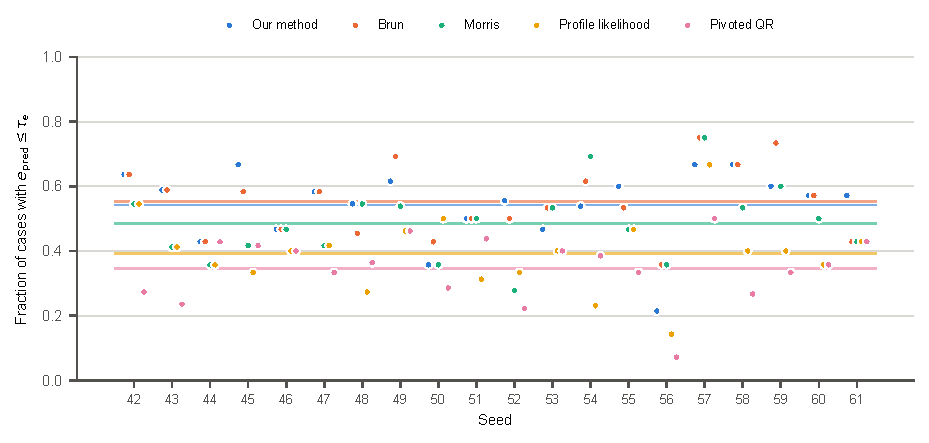
\includegraphics[width=\textwidth]{figures/figS_synth_semillas.pdf}
\caption{\textbf{Synthetic experiment: fraction of cases with $e_{\mathrm{pred}}\le\tau_e$ for each criterion and seed.} Horizontal lines, mean over seeds. Cases common to the five criteria with signal.}
\label{fig:synthsemillas}
\end{figure}
